\section[Horizonte infinito]{Análisis de Simulación con horizonte infinito}

\begin{frame}{Análisis de Simulación con horizonte infinito}
    \begin{itemize}
        \item Existen dos métodos básicos para desarrollar simulaciones con estado estable:
        \begin{enumerate}
            \item Correr múltiples réplicas. 
            \item Correr una sola réplica muy larga. 
        \end{enumerate}
        \item Ambos métodos dependen del manejo de los aspectos no estacionarios de los datos.
    \end{itemize}
\end{frame}

\begin{frame}{Análisis de Simulación con horizonte infinito}

    \begin{itemize}
        \item Al analizar simulaciones con horizonte infinito, la principal dificultad es la naturaleza de los datos dentro de las réplicas.
        \item El análisis estadístico suele requerir:
        \begin{enumerate}
            \item Observaciones independientes.
            \item Observaciones tomadas de distribuciones idénticas.
            \item Observaciones extraídas de una distribución normal (o que haya suficientes observaciones para recurrir al teorema del límite central).
        \end{enumerate}
        \item Las salidas dentro de una réplica no satisfacen ninguna de esas condiciones; sin embargo, ciertos procedimientos pueden establecerse en la forma en que se toman los datos para asegurar que los supuestos no sean gravemente violados.
    \end{itemize}
\end{frame}

%Effect of initial conditions
\begin{frame}{Efecto de las condiciones iniciales}
    \begin{itemize}
        
        \item Sea $F_i(x|I)$ la distribución condicional acumulada de $X_i$ donde $I$ representa las condiciones utilizadas al iniciar la simulación en el tiempo 0. 
        \item Si $F_i(x|I)\rightarrow F(x)$ cuando $i \rightarrow \infty$, para cualquier $I$, entonces $F(x)$ se denomina la distribución de estado estable del proceso. 
        \item Las condiciones iniciales de una simulación, representan el estado del sistema cuando la simulación comienza.
    \end{itemize}
\end{frame}

\begin{frame}{Efecto de las condiciones iniciales}
    \begin{itemize}
        \item La dificultad al estimar el desempeño en estado estable, es que al menos que el sistema inicie utilizando la distribución de estado estable (la cual no se conoce), no hay forma de observar directamente la distribución de estado estable.
        \item La distribución $F_i(x|I)$ al comienzo de la simulación depende fuertemente de las condiciones iniciales.
        \item Si la distribución de estado estable existe, al correr una simulación suficientemente larga, los estimadores tienden a converger a las cantidades deseadas.
    \end{itemize}
\end{frame}

\begin{frame}{Efecto de las condiciones iniciales}{Estado transitorio y estable}
    \begin{figure}
        \centering
        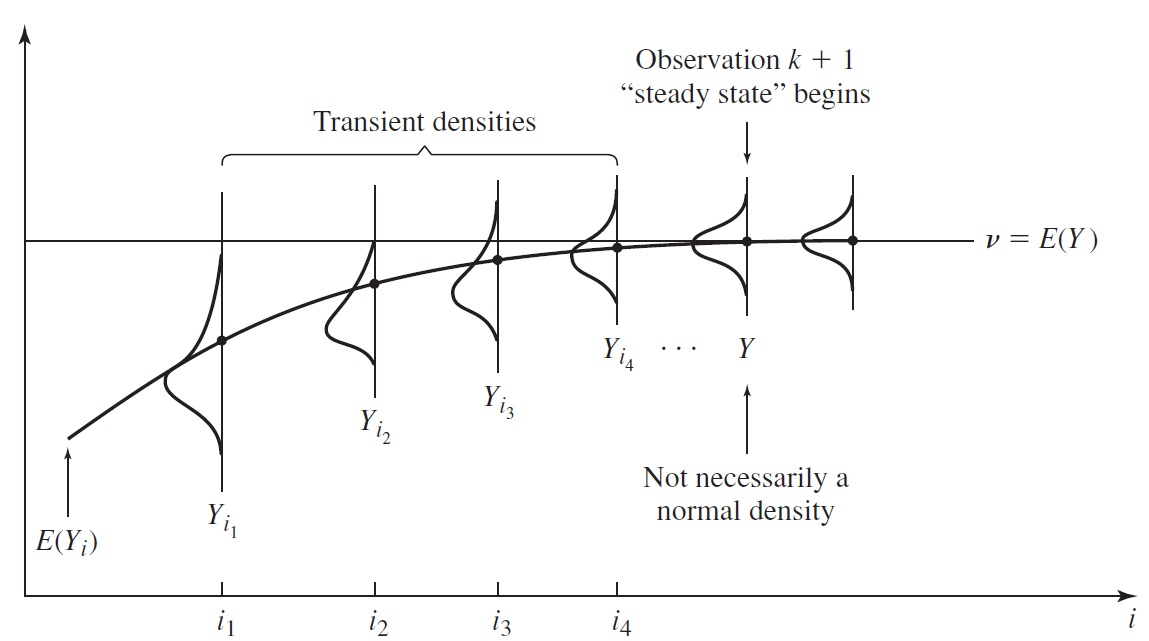
\includegraphics[width=8cm]{images/transientSteadyState.jpg}
        %\caption{Caption}
        \label{fig:TransientSteadyState}
    \end{figure}
\end{frame}

\begin{frame}{Efecto de las condiciones iniciales}
    \begin{itemize}
        \item Los estimadores de las medidas de desempeño en estado estable como los promedios muestrales tenderán a estar \textit{sesgados}. 
        \item Un estimador, $\hat{\theta}$, es un estimador \textit{insesgado} de un parámetro de interés $\theta$, si $E[\hat{\theta}]=\theta$.
        \item Si el estimador es sesgado, entonces la diferencia, $E[\hat{\theta}-\theta]$, se denomina el sesgo del estimador $\hat{\theta}$.
        \item El sesgo es una propiedad del estimador. Para estimar el sesgo de un estimador, se requiere contar con múltiples observaciones del estimador.
    \end{itemize}
\end{frame}

\begin{frame}{Periodo de calentamiento}
    \begin{itemize}
        \item Para mitigar el \textit{sesgo de inicialización}, aquel producido por la elección de unas condiciones iniciales específicas diferentes de $F(x)$, se puede emplear un método de simulación en dos fases.% conocido como \textit{periodo de calentamiento}.
        \item La estrategia consiste en encontrar un índice $d$, para el proceso de salida $X_i$, tal que $X_i; i=d+1, \dots$ tenga en esencia las mismas propiedades que la distribución en estado estable $F(x)$.
        \item Donde, $i=1,\dots, d$ es el \textit{periodo de calentamiento} del sistema y no se consideran para el cálculo de los estimadores. De esta forma, los estimadores de desempeño en estado estable se basan solo en $X_i;i=d+1, \dots$. 
    \end{itemize}
\end{frame}

\begin{frame}{Periodo de calentamiento}
    \begin{figure}
        \centering
        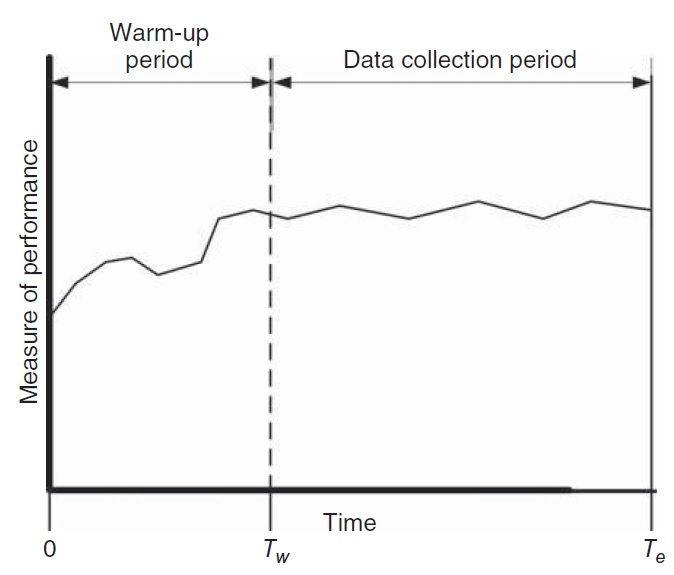
\includegraphics[width=8cm]{images/steady_state.jpg}
        %\caption{Caption}
        %\label{fig:my_label}
    \end{figure}
\end{frame}

\begin{frame}{Periodo de calentamiento}
    \begin{itemize}
        \item Varios métodos y políticas se han propuesto para determinar el periodo de calentamiento.
        \item Se explica a continuación un procedimiento gráfico:
            \begin{enumerate}
                \item Realice $n$ réplicas (se recomienda $n>5$).
                \item Sea $Y_{rj}$ la $j$-ésima observación en la réplica $r$, para $j=1,2,\dots,m_r$, donde $m_r$ es el número de observaciones en la réplica $r$.
                \item Calcule el promedio a través de cada réplica para cada $j=1,2,\dots,m$, donde $m=\min(m_r$, para $r=1,2,\dots,n$
                \[\bar{Y_{\cdot j}}=\frac{1}{n}\sum_{r=1}^{n}{Y_{rj}}\]
                \item Grafique $\bar{Y_{\cdot j}}$ para cada $j=1,2,\dots,m$.
                \item Evalúe visualmente dónde las gráficas comienzan a converger.
            \end{enumerate}
    \end{itemize}

\end{frame}

%Method of replication-deletion
\begin{frame}{Método de replicación-eliminación}
    \begin{itemize}
        \item Al realizar simulación de horizonte infinito especificando un periodo de calentamiento y haciendo múltiples réplicas, se emplea el \textit{método de replicación-eliminación}.
        \item Este método es muy utilizado en la práctica por la simplicidad del análisis después de que se ha determinado un periodo de calentamiento adecuado.
    \end{itemize}
\end{frame}

\begin{frame}{Método de replicación-eliminación}
    \begin{itemize}
        \item Al eliminar las estadísticas durante el periodo de calentamiento se reduce el sesgo de inicialización.
        \item Existe una compensación entre la variabilidad del estimador y el sesgo de inicialización. 
        \item Al eliminar parte de los datos, al variabilidad del estimador tiende a subir cuando el sesgo de inicialización disminuye.
    \end{itemize}
\end{frame}
    
\begin{frame}{Método de replicación-eliminación}
    \begin{itemize}
        \item En cada réplica, parte de los datos se desecha. Lo cual representa tiempo computacional que podría ser usado más eficientemente recolectando datos útiles.
        \item Las técnicas para determinar el periodo de calentamiento (como el procedimiento gráfico) requieren por lo general almacenar una cantidad significativa de datos.
    \end{itemize}
\end{frame}

\begin{frame}{Método de replicación-eliminación}
    \begin{itemize}
        \item Si se tienen múltiples medidas de desempeño, es posible que se requiera desarrollar un análisis del periodo de calentamiento por cada una, ya que cada medida de desempeño puede converger al estado estable a una tasa diferente.
        \item En tal caso, el periodo de calentamiento debe ser lo suficientemente grande como para cubrir todas las medidas de desempeño.
        \item De no especificarse un periodo de calentamiento suficientemente largo, es posible que esté agravando el problema del sesgo para las $n$ réplicas.
    \end{itemize}
\end{frame}

    %Batch means
\begin{frame}{Método de lotes equivalentes}
    \begin{itemize}
        \item En el método de los lotes equivalentes, solo se corre una réplica.
        \item Después de eliminar el periodo de calentamiento, el resto de la corrida es dividida en $k$ lotes, donde el promedio en cada lote representa una observación.
    \end{itemize}
\end{frame}

%As previously mentioned, the method of replication–deletion causes each replication to delete the initial portion of the run. As an alternative, you can make one long run and delete the initial portion only once. When analyzing an infinite-horizon simulation based on one long replication, a method is needed to address the correlation present in the within-replication data.

\begin{frame}{Método de lotes equivalentes}
    \begin{figure}
        \centering
        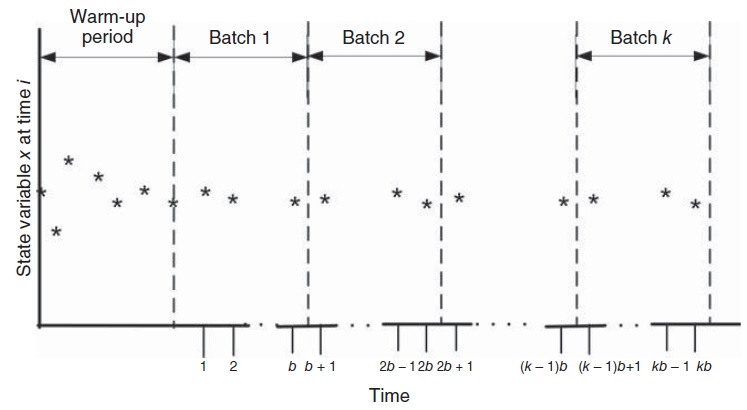
\includegraphics[width=10cm]{images/batch_means.jpg}
        %\caption{Caption}
        \label{fig:my_label}
    \end{figure}
\end{frame}

\begin{frame}{Método de lotes equivalentes}
    \begin{itemize}
        \item La ventaja de este método es que comprende una réplica muy larga, moderando el efecto de las condiciones iniciales.
        \item La principal desventaja es que las observaciones dentro de la réplica estás correlacionadas y a menos que se formen adecuadamente, los lotes pueden exhibir un fuerte grado de correlación.
    \end{itemize}
\end{frame}

\begin{frame}{Método de lotes equivalentes}
    \begin{itemize}
        \item El principal problema en este método es determinar el tamaño del lote o de forma alternativa el número de lotes a utilizar.
        \item Lotes más largos mejoran la independencia de las observaciones, pero reduce el número de lotes, resultando en una mayor varianza del estimador.
    \end{itemize}
\end{frame}